\documentclass{beamer}

\usepackage[utf8]{inputenc}
\usepackage{default}
\usepackage{graphicx}
\usepackage{epstopdf}
\graphicspath{ {imagenes/} }

\usetheme{Warsaw}
\usecolortheme{crane}
\useoutertheme{shadow}
\useinnertheme{rectangles}

\title{Aumenting Data Structures}

\author{Chris Chávez}
\institute{Universidad Nacional de San Agustín - Escuela Profesional de Ciencia de la Computación}
\date{\today}

\begin{document}

\frame{\titlepage}

\begin{frame}
 \frametitle{Order Statistics Tree}
 \begin{itemize}
  \item The $i^{th}$ order statistic of a set of $n$ elements, where $i \epsilon \{1,2,...,n\}$, is
  simply the element in the set with the $i^{th}$ smallest key.
  \item Compute the \textbf{rank} of an element in $O(lg n)$ time.
 \end{itemize}
\end{frame}

\begin{frame}
 \begin{figure}
  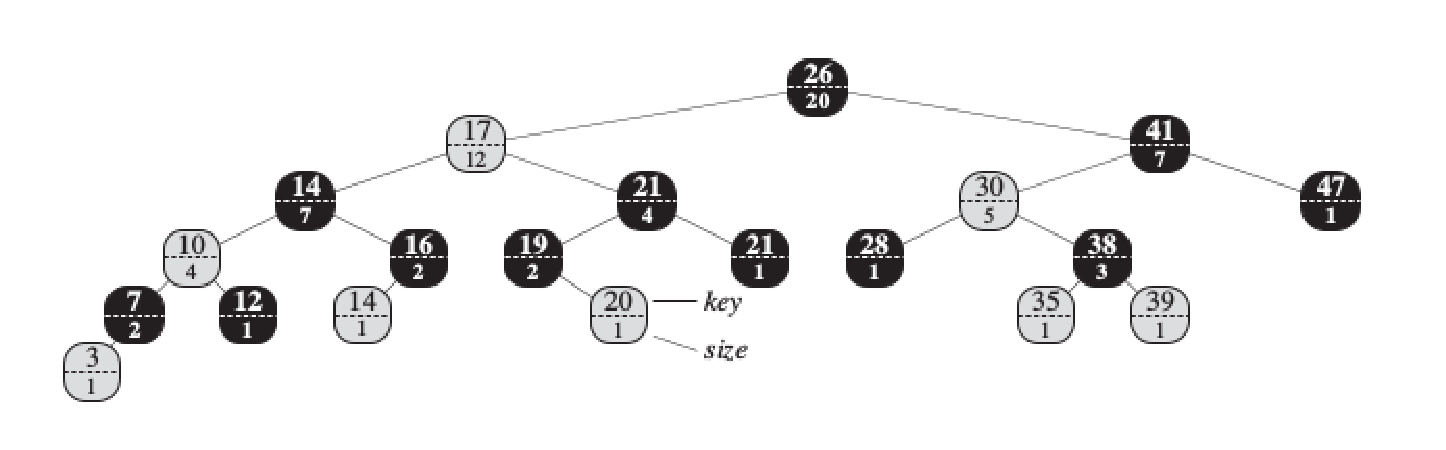
\includegraphics[scale=0.45]{1.eps}
 \end{figure}
\end{frame}

\begin{frame}
 \begin{figure}
  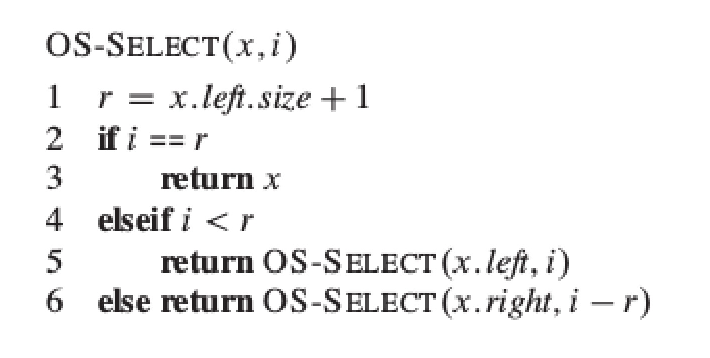
\includegraphics[scale=0.7]{2.eps}
 \end{figure}
\end{frame}

\begin{frame}
 \begin{figure}
  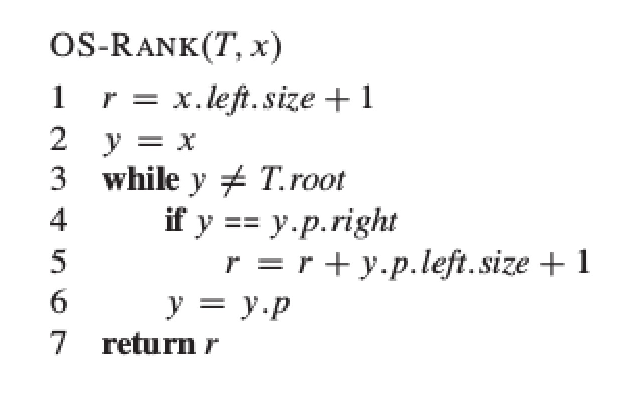
\includegraphics[scale=0.7]{3.eps}
 \end{figure}
\end{frame}

\begin{frame}
 \frametitle{Maintaining subtree sizes}
 \begin{itemize}
  \item \textbf{Step 1:} We simply increment $x.size$ for each node $x$ on the simple path traversed from the root down toward
  the leaves.
  \item \textbf{Step 2:}
   \begin{figure}
    \includegraphics[scale=0.6]{4.eps}
   \end{figure}
 \end{itemize}
\end{frame}

\begin{frame}
 \begin{figure}
  \includegraphics[scale=0.6]{5.eps}
 \end{figure}
\end{frame}

\begin{frame}
 \frametitle{How to augment a data structure}
 \begin{enumerate}
  \item Choose an underlying data structure.
  \item Determine additional information to maintain int hte underlying data structure.
  \item Verify that we can maintain the additional information for the basic modifying operations on the
  underlying data structure.
  \item Develop new operations.
 \end{enumerate}

\end{frame}






\end{document}
